\chapter{Analisi dinamica}

Questa viene fatta per ora in locale.

\section{Cuckoo Sandbox}
Sandbox per fare le nostre analisi.
Come funziona?

\subsection{Architettura applicata}
Virtualbox, con altro Virtualbox; in locale.

\begin{figure}[H]
    \centering
    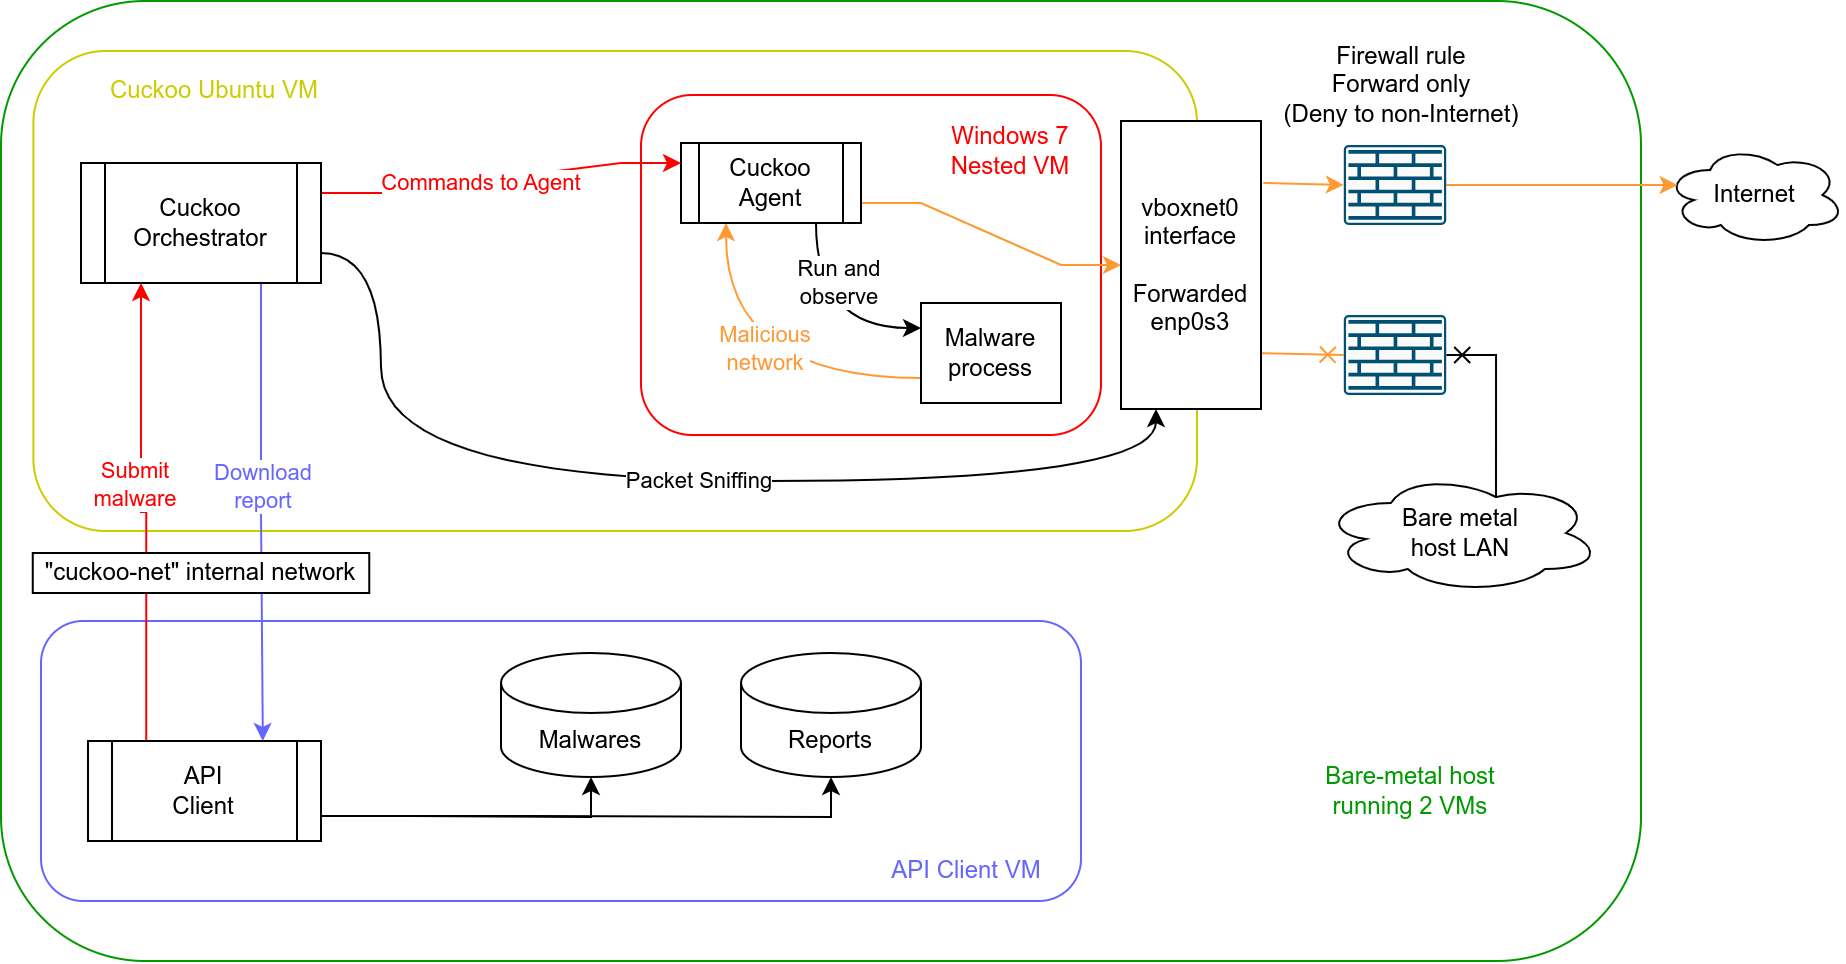
\includegraphics[width=\textwidth]{assets/cuckoo_vms.png}
    \caption{Architettura dell'infrastruttura di analisi dinamica}
    \label{fig:cuckoo_vms_architecture}
\end{figure}

\subsection{Setup con systemd e Docker}
Perchè?
\begin{itemize}
    \item Docker perché così vado ad avviare i vari servizi secondari necessari come Mongo o PostgreSQL
    \item Systemd per l'avvio automatico del servizio, così da essere subito operativo
    \item \textbf{Problemi?} Certo, tanti appunti su Obsidian
\end{itemize}

\section{Hardening}

\section{Anti-VM detection}
Pafish, vediamo la differenza tra VM standard (fig. \ref{fig:pafish_standard_vm}) e Cuckoo (fig. \ref{fig:pafish_cuckoo}) con le sue tecniche anti-VM:

\begin{figure}[H]
\centering
\begin{subfigure}{.5\textwidth}
  \centering
  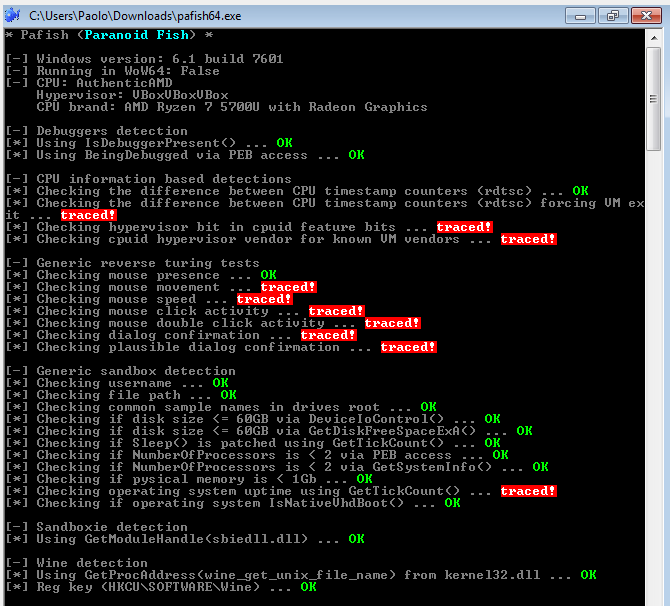
\includegraphics[width=.9\linewidth]{assets/pafish_standard_vm_1.png}
\end{subfigure}%
\begin{subfigure}{.5\textwidth}
  \centering
  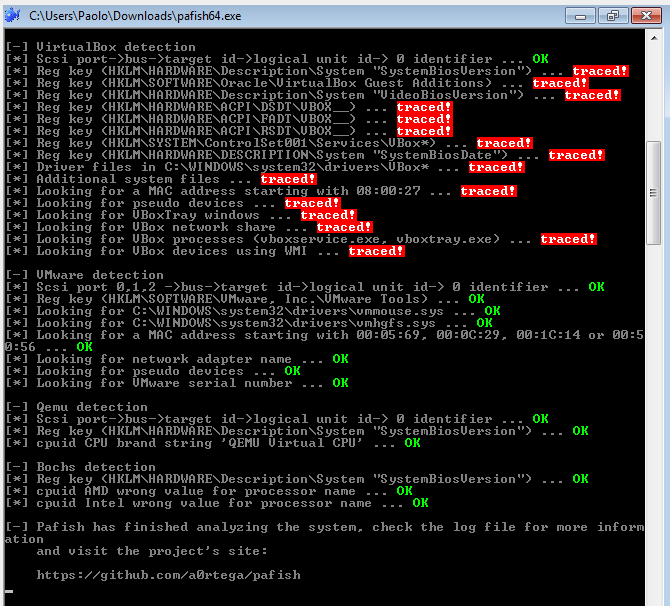
\includegraphics[width=.9\linewidth]{assets/pafish_standard_vm_2.png}
\end{subfigure}
\caption{Pafish eseguito in una classica VM Windows 7}
\label{fig:pafish_standard_vm}
\end{figure}

\begin{figure}[H]
\centering
\begin{subfigure}{.5\textwidth}
  \centering
  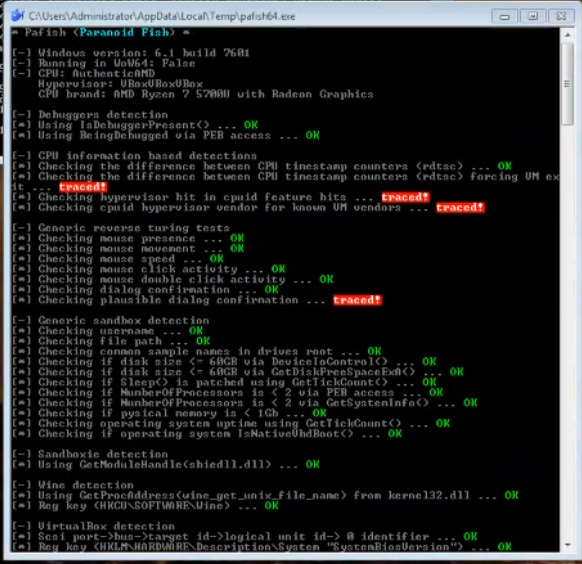
\includegraphics[width=.9\linewidth]{assets/pafish_cuckoo_1.png}
\end{subfigure}%
\begin{subfigure}{.5\textwidth}
  \centering
  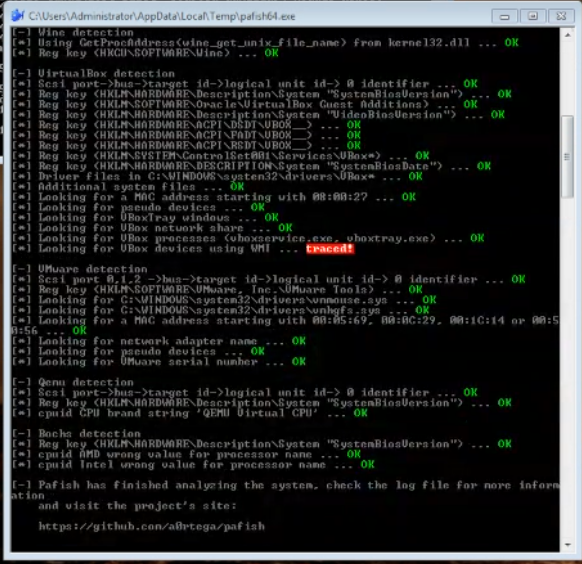
\includegraphics[width=.9\linewidth]{assets/pafish_cuckoo_2.png}
\end{subfigure}
\caption{Pafish eseguito sotto l'analisi di Cuckoo Sandbox}
\label{fig:pafish_cuckoo}
\end{figure}

\section{Workflow analisi dinamica}
